\chapter{Analisi del progetto di tirocinio}
\section{Introduzione}
In questo capitolo ci dedicheremo a dare uno sguardo all'architettura prototipale proposta come prodotto del tirocinio curriculare. Forniremo una panoramica generale dell'architettura, descrivendo i progetti che costituiscono la soluzione complessiva ("progetto" e "soluzione" appartengono alla terminologia specifica nel contesto di uno sviluppo di Visual Studio in ambiente .NET) e il loro ruolo rispetto al resto dell'architettura. Si avrà inoltre cura di giustificare le scelte implementative effettuate, con riferimento a o in contrasto con alla teoria e i principi di progettazione esposti nel terzo capitolo. Si ribadisce infatti come la soluzione proposta sia un prototipo, e in quanto tale devia consapevolmente dall'idea platonica del prodotto adatto alla produzione per assecondare vincoli di tempo e risorse inevitabili in un contesto di sviluppo con finalità didattiche. Nei casi in cui un aspetto dell'implementazione si discosti dai principi di buona progettazione delle architetture a microservizi, verrà prontamente indicato l'approccio che, in un contesto di sviluppo professionale, si sarebbe invece adottato, eventualmente descrivendo i \emph{trade-off} dell'impiego dell'una o dell'altra implementazione.

\section{Panoramica della soluzione}
La soluzione complessiva si articola in quattro progetti principali, realizzati con tecnologia \emph{ASP.NET Core} in \emph{.NET 8 \emph{(nuovo, supporto a lungo termine)}}, che rappresentano i microservizi forniti dall'architettura, e tre progetti secondari, rispettivamente una libreria di utility, un progetto condiviso \emph{.NET} per la definizione di modelli di dati condivisi, e il progetto Docker Compose per la gestione automatica e centralizzata dei container che ospitano i microservizi.

Si segnala nella struttura descritta una scelta di progettazione, consciamente non in linea con i principi di incapsulamento e indipendenza dei microservizi, effettuata per snellire un'architettura che sarebbe altrimenti eccessivamente complessa per il numero di servizi principali forniti. Un microservizio fa da gateway API e comunica con l'esterno, mentre esso e gli altri microservizi comunicano fra loro in una rete Docker privata di tipo \texttt{bridge}. Ogni microservizio stateful utilizza per la persistenza un database SQLite: questa soluzione, pur non scalabile, è stata adottata per la semplicità di configurazione e gestione in un contesto prototipale, in cui scalabilità, efficienza e sicurezza non valgono l'impegno nell'impostare un sistema di gestione più complesso in assenza di parametri di scelta che sarebbero invece centrali in un contesto professionale e di produzione.

Una progettazione più rigorosa avrebbe richiesto un microservizio a sé stante che ospitasse il motore di generazione di reportistica ed esponesse il servizio verso i microservizi a gestione del client MVC e della Web API. Nel contesto di tale scelta, il contenuto del progetto condiviso \emph{UserDocuments} sarebbe inglobato nel microservizio di reportistica, non necessitando Web API e client MVC di conoscere il modello di dati dei documenti generati.
La soluzione prototipale prevede invece l'inclusione del motore di reportistica all'interno del microservizio per la Web API: la generazione di nuovi report è infatti limitata a tale container (il client MVC esegue un redirecting verso di esso, così da non esporre al browser endpoint diversi con lo stesso scopo finale), mentre l'accesso al sistema di storage dei report è condiviso mediante un \emph{named volume} Docker, a sottolineare la provvisorietà di tale soluzione nel contesto di un progetto con prospettive di sviluppo in direzione di un deploy in ambienti distribuiti.

\begin{figure}[H]
    \centering
    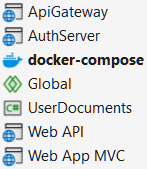
\includegraphics[width=0.4\textwidth]{fig/elenco_progetti.png}
    \caption[Elenco progetti]{Elenco dei progetti che compongono il codice sorgente della soluzione}
\end{figure}

\subsection{Gateway API}
Il progetto \emph{APIGateway} implementa il pattern omonimo nel contesto della soluzione proposta. Si tratta di un microservizio \emph{ASP.NET Core} che funge da SPoA (\emph{Single Point of Access}) per l'architettura, fornendo funzionalità di \emph{reverse proxying} grazie all'impiego del pacchetto \emph{YARP} e di centralizzazione dell'autenticazione con refresh intelligente dei token.

\emph{YARP} (\emph{Yet Another Reverse Proxy}) è un framework open-source per la creazione di proxy HTTP, sviluppato e mantenuto da Microsoft, che consente di instradare le richieste in ingresso verso uno o più servizi backend in modo flessibile e configurabile. Gran parte delle specifiche di instradamento, infatti, sono state definite direttamente come oggetto all'interno nel file di configurazione del progetto .NET (che per default è nominato \emph{appsettings.json}), mentre le richieste di Logout, che implementano una logica più avanzata per l'invalidazione di cookie e token e per il sign out dal contesto dell'Identity, sono state configurate all'interno del middleware nel file di avvio del progetto \emph{Program.cs}.

L'approccio di estrarre le informazioni variabili in un file di configurazione non riguarda soltanto il routing del reverse proxy, ma è adottato in maniera consistente nei progetti .NET dell'intera applicazione, consentendo non solo di mantenere un file di avvio snello e facilmente leggibile, ma anche di centralizzare la gestione delle configurazioni grazie all'elasticità fornita dall'ambiente \emph{.NET}.
Tali dati sono infatti estratti mediante un oggetto \texttt{ConfigurationManager}, che rappresenta un unico punto d'accesso alle configurazioni, dotato di un sistema di priorità e di metodi per lo strong typing dei valori ottenuti. Per accesso con priorità si intende che il \texttt{ConfigurationManager} di un applicazione ASP.NET è in grado di ricercare le configurazioni richieste da più fonti in una gerarchia stabilita, consentendo allo sviluppatore di specificare override diversi in \emph{environment} diversi (sviluppo, testing, produzione) ed eventualmente di iniettare la configurazione come variabili d'ambiente mediante Docker, semplificando notevolmente il deploy in ambienti distribuiti in cui, ad esempio nel caso del gateway API, è necessario specificare all'avvio le informazioni sulla rete in cui il servizio viene installato.

L'altra funzionalità importante fornita dal progetto \emph{APIGateway} è la gestione centralizzata dell'autenticazione e dell'autorizzazione degli utenti, implementando il pattern \emph{Authentication Gateway}.

Al momento di una richiesta da parte di un client, il gateway verifica che l'utente sia autenticato prima che la richiesta raggiunga i microservizi interni e, in caso contrario, lo ridireziona all'apposita interfaccia grafica fornita dal microservizio AuthServer, che analizzeremo in seguito (se la richiesta è programmatica restituisce invece \texttt{Error 401}): una volta autenticato, all'utente sono associati un token JWT (JSON Web Token) e un cookie, che il gateway provvederà ad inoltrare ai microservizi backend e a rinnovare periodicamente in modo trasparente per l'utente: il token JWT e il cookie consentono all'utente di autenticarsi una volta sola (presso il gateway) e restare connesso per l'uso di Web API e client MVC rispettivamente.

\subsection{AuthServer}
Il progetto \emph{AuthServer} descrive il microservizio che fa da Identity Provider per l'applicativo. Utilizza il framework \emph{Duende Identity Server} per implementare e configurare con pochi metodi un servizio di autenticazione completo basato sul protocollo OpenID Connect. Per la gestione di utenti e ruoli si affida invece ad \emph{Identity} con \emph{EntityFramework Core}: grazie alla potenza e l'interazione \emph{seamless} dei framework, in questo progetto la persistenza è stata gestita in maniera potente ed integrata senza dover scrivere una sola riga di codice \emph{SQL} o dover configurare manualmente il database (qui SQLite ospitato su un \emph{named volume Docker}, configurazione accettabile in un ambiente prototipale per motivazioni discusse in precedenza). Si pensi che l'intera configurazione dell'Identity Server con le funzionalità essenziali (2FA, login con provider esterni o email sender sarebbero inutili in un contesto prototipale offline) è stata realizzata con l'invocazione di meno di 7 metodi nell'entrypoint del servizio (\emph{Program.cs}).
\begin{figure}[H]
        \centering
        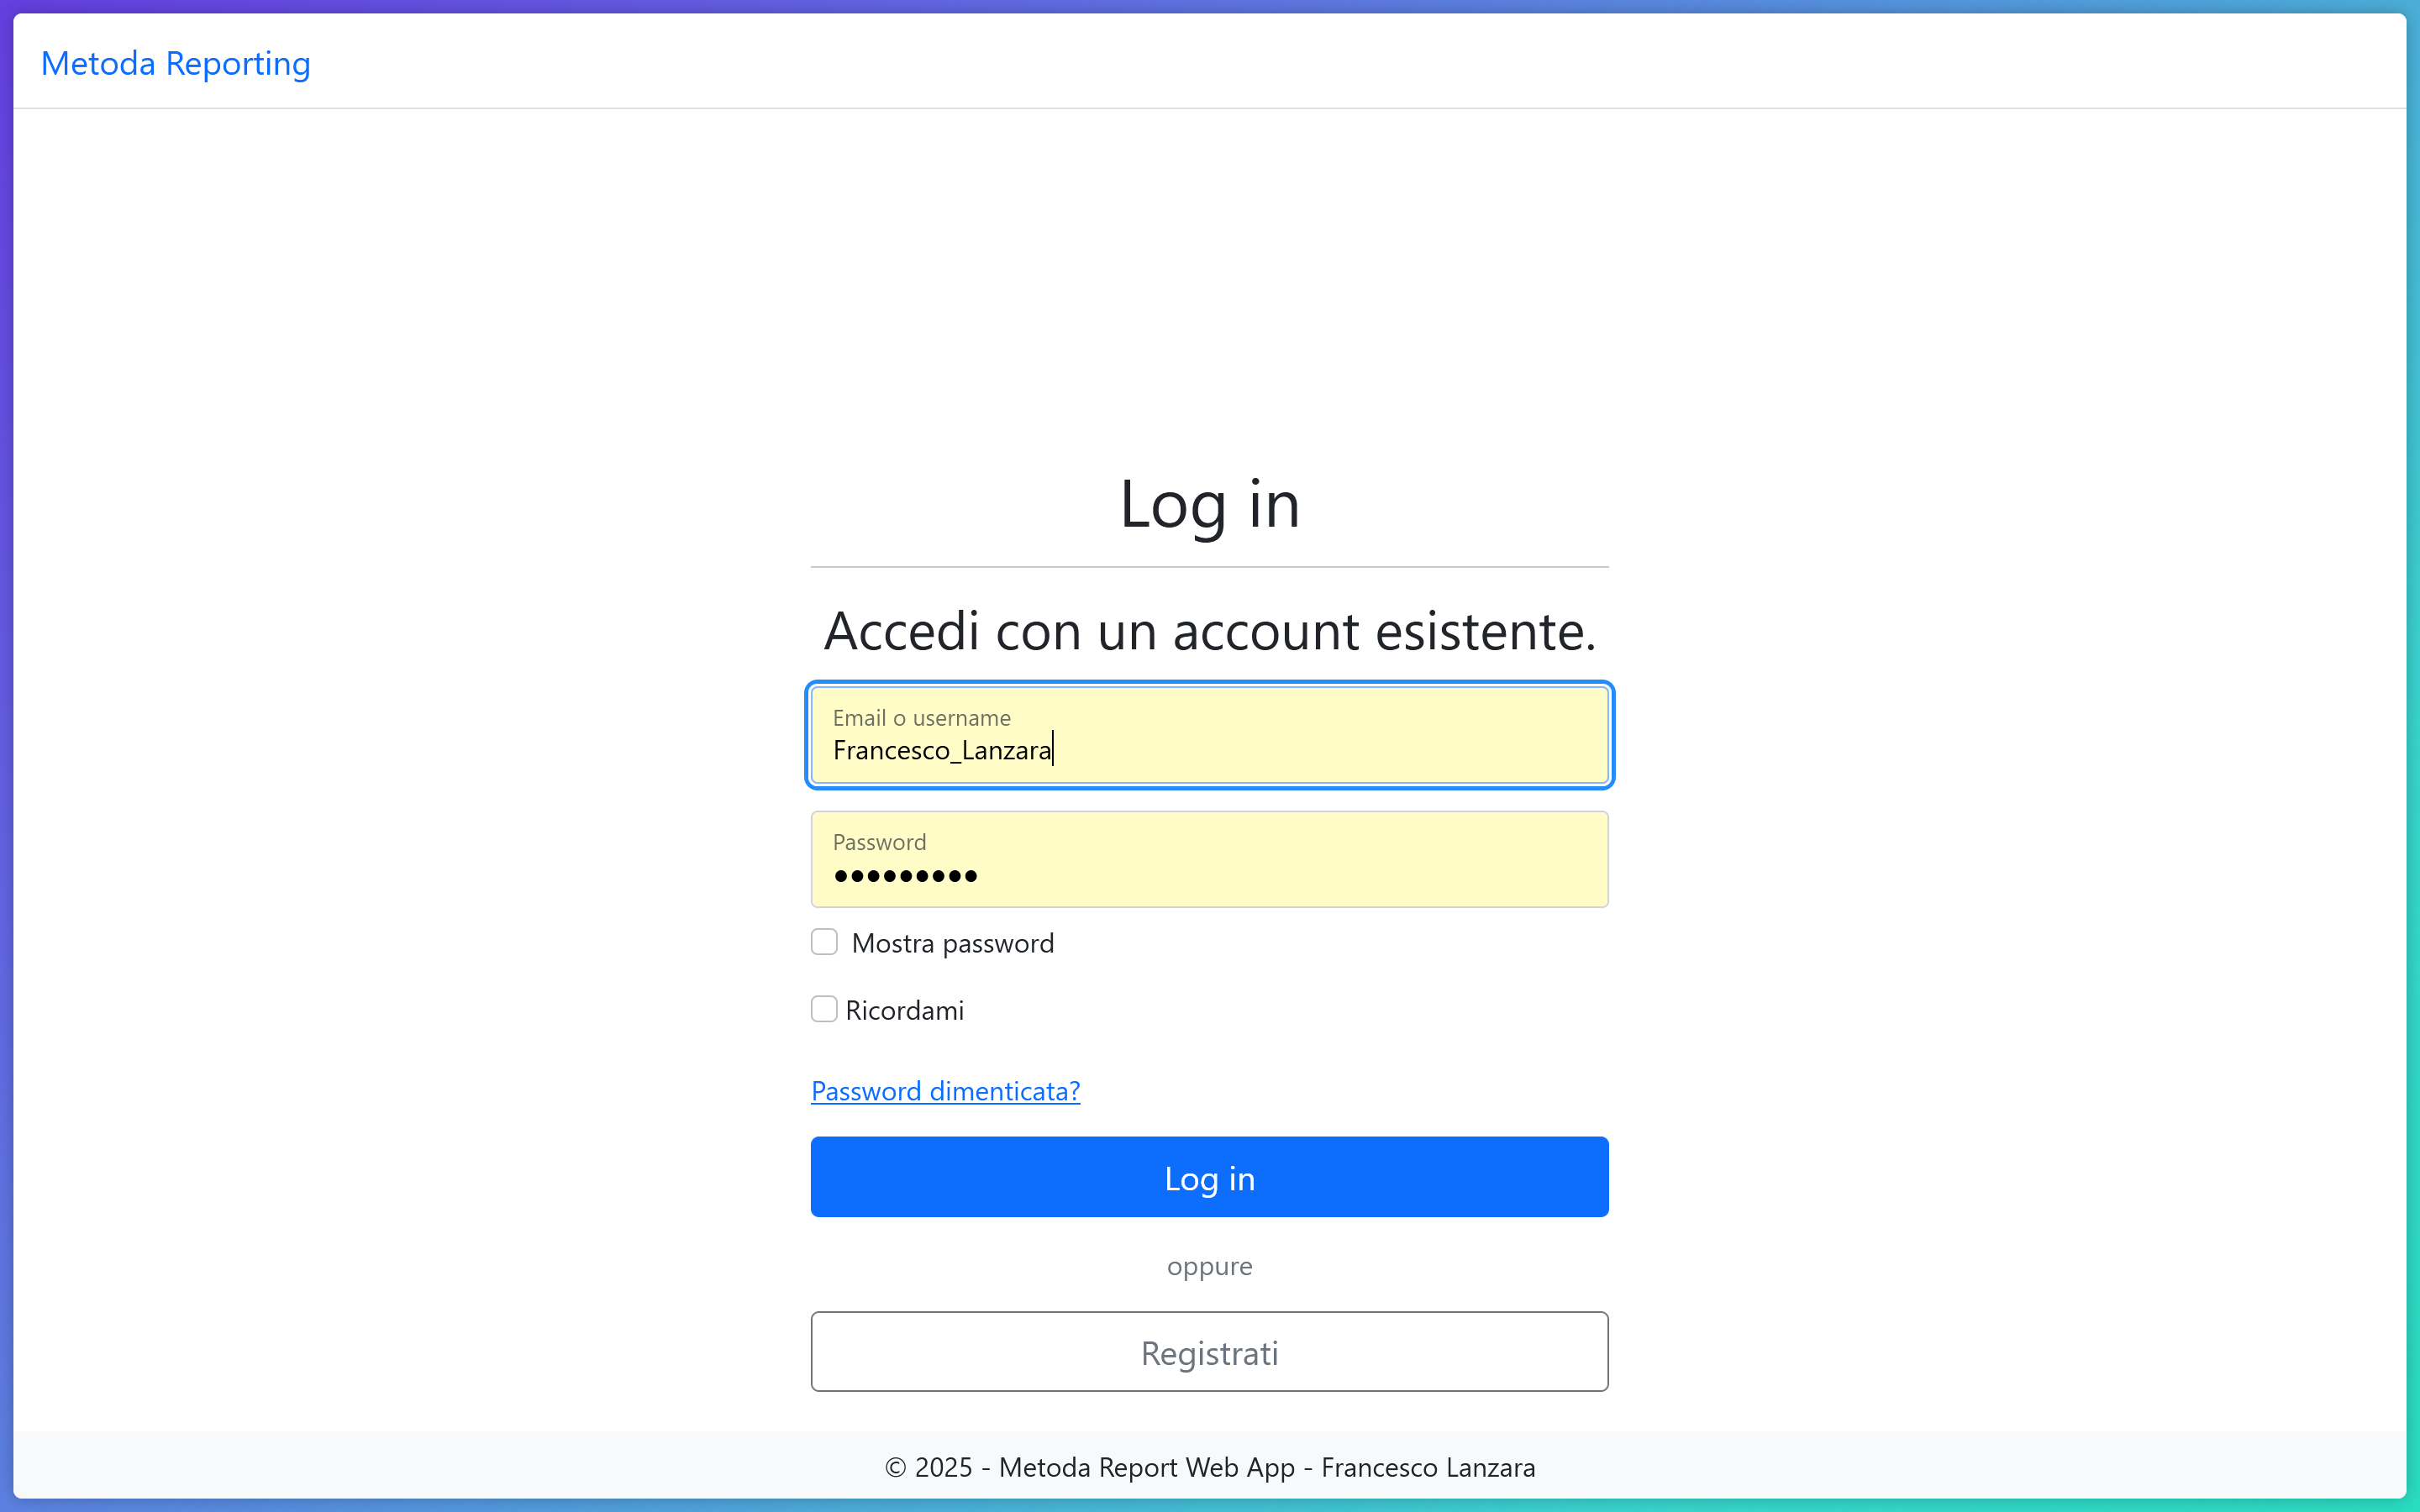
\includegraphics[width=15.5cm]{fig/screen_login.png}
        \caption[Schermata login]{La schermata di login. Da questa schermata è possibile accedere anche alla registrazione e al recupero della password.}
\end{figure}
Il sistema di scaffolding .NET, che consente la generazione automatica di codice \emph{boilerplate} per la configurazione rapida delle funzionalità offerte dai framework, è stato utilizzato per generare la struttura alla base del rendering delle pagine di accesso, registrazione e gestione del profilo utente, che sono state poi personalizzate per adattarle alle esigenze del progetto e rese gradevoli alla vista con classi del framework \emph{Bootstrap} per \emph{CSS}.
Si tenga conto che nonostante la scelta, analizzata nel capitolo quarto, di implementare l'interfaccia grafica della web app mediante ASP.NET Core MVC, l'implementazione di base generata per interfaccia di autenticazione fa utilizzo della tecnologia \emph{Razor Pages}, che adotta un approccio \emph{MVVC}-like, basato sul concetto di \emph{PageModel}, associando a ogni pagina \texttt{.cshtml} un file \emph{.cs} che ne descrive la logica e il modello: il risultato è una struttura più fluida e meno verbosa che fa largo uso di convenzioni, rendendo semplice implementare funzionalità comuni ma risultando nel complesso meno flessibile di MVC.
\begin{figure}[H]
        \centering
        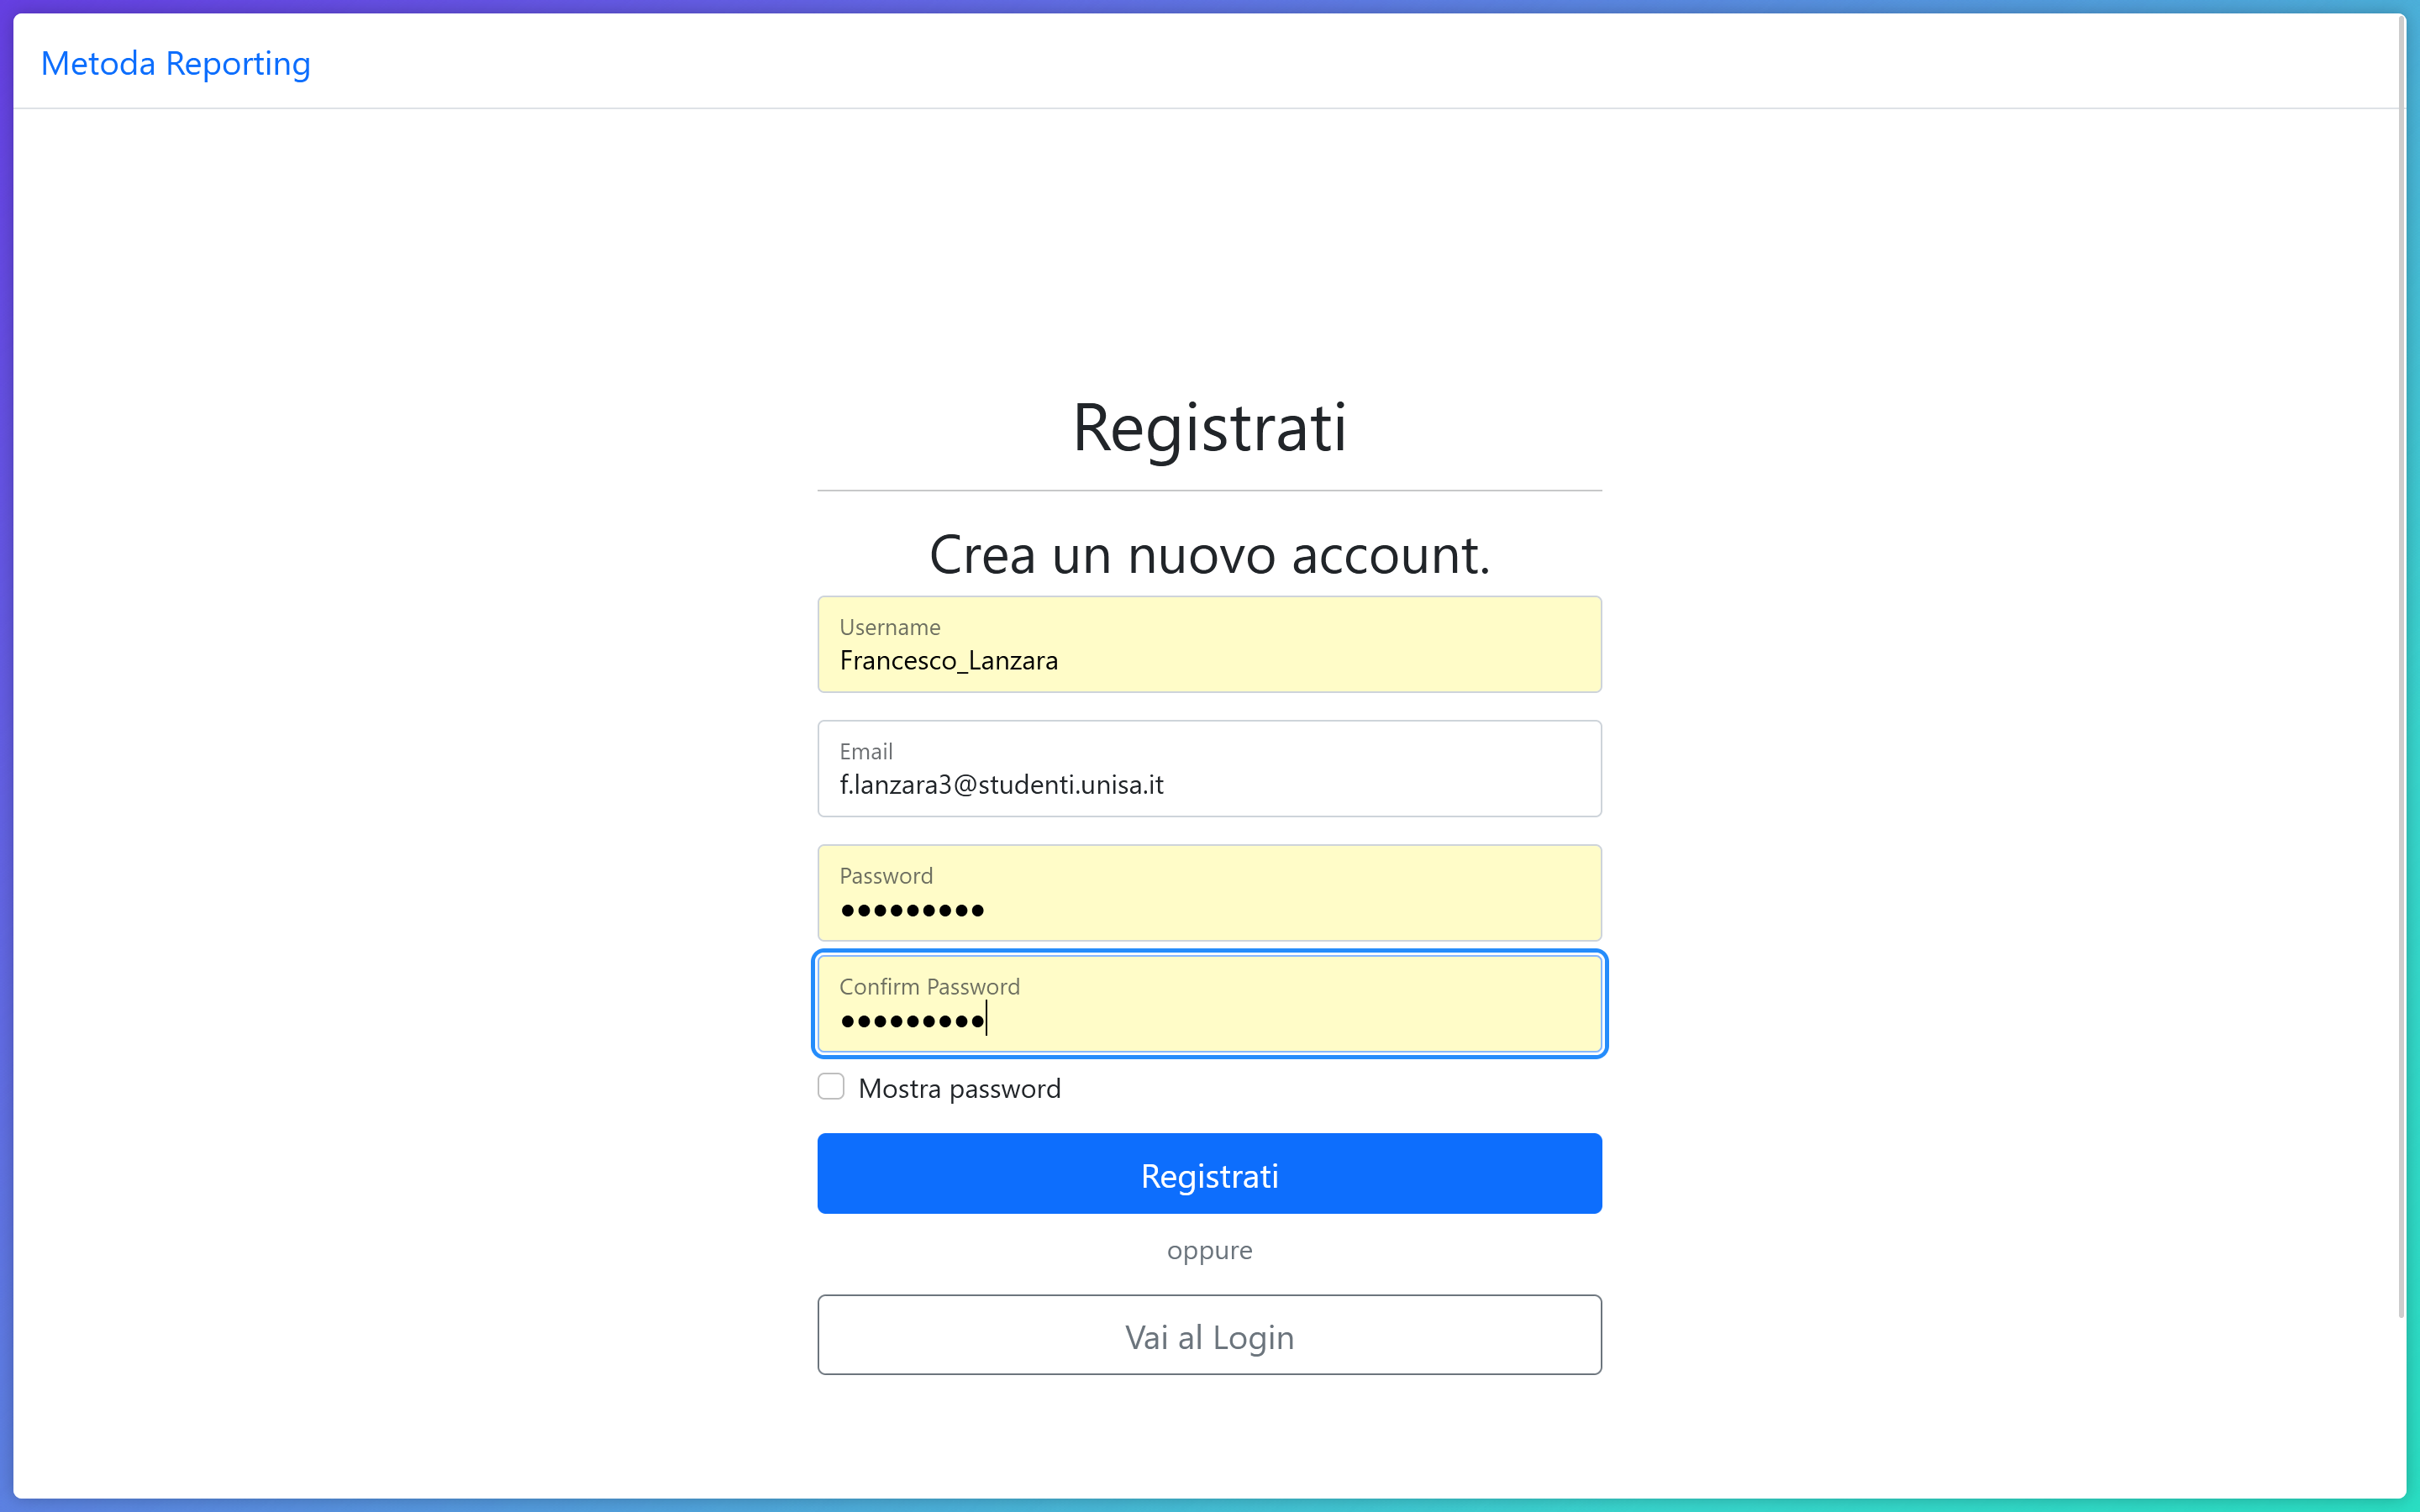
\includegraphics[width=15.5cm]{fig/screen_register.png}
        \caption[Schermata registrazione]{La schermata di registrazione. Da questa schermata è possibile tornare al login.}
\end{figure}
Dal momento che la logica di autenticazione è gestita internamente lontano dagli occhi dello sviluppatore, il sottoscritto ha ritenuto preferibile mantenere l'implementazione già predisposta, limitandosi a personalizzare aspetto e interazione delle pagine, piuttosto che impiegare tempo per individuare una soluzione alternativa nel tentativo di mantenere coerenza con una scelta implementativa che riguarda un altro microservizio dell'architettura. In un contesto in cui un controllo chiaro sull'implementazione non è ottenibile indipendentemente dalla tecnologia impiegata, il vantaggio principale del pattern MVC viene meno, giustificando ulteriormente la scelta di adottare Blazor per l'AuthServer.

AuthServer si occupa dunque di rispondere alle richieste di autenticazione e fornire le schermate per il login, la registrazione ed altre funzionalità legate all'account, come reset e modifica della password, gestione di altre informazioni del profilo quali recapiti telefonico e mail, logout. Si tenga conto che un utente già autenticato può accedere a queste pagine senza perdere l'accesso, ritornando all'applicazione MVC tramite click sul nome del servizio (estremo sinistro del layout superiore).
Esso espone inoltre gli endpoint necessari per il protocollo OpenID Connect, che consente ai client di autenticare gli utenti e ottenere informazioni sui loro profili in modo sicuro e standardizzato. Tali endpoint sono utilizzati dal gateway API per autenticare gli utenti che tentano di accedere ai microservizi protetti dell'architettura.
L'accesso dell'utente mediante \emph{OpenID Connect} fornisce al browser un cookie di sessione e un codice, che il gateway (punto di accesso dell'utente) utilizza per ottenere un token JWT, inoltrato alla Web API per autorizzare delle richieste.
\begin{figure}[H]
        \centering
        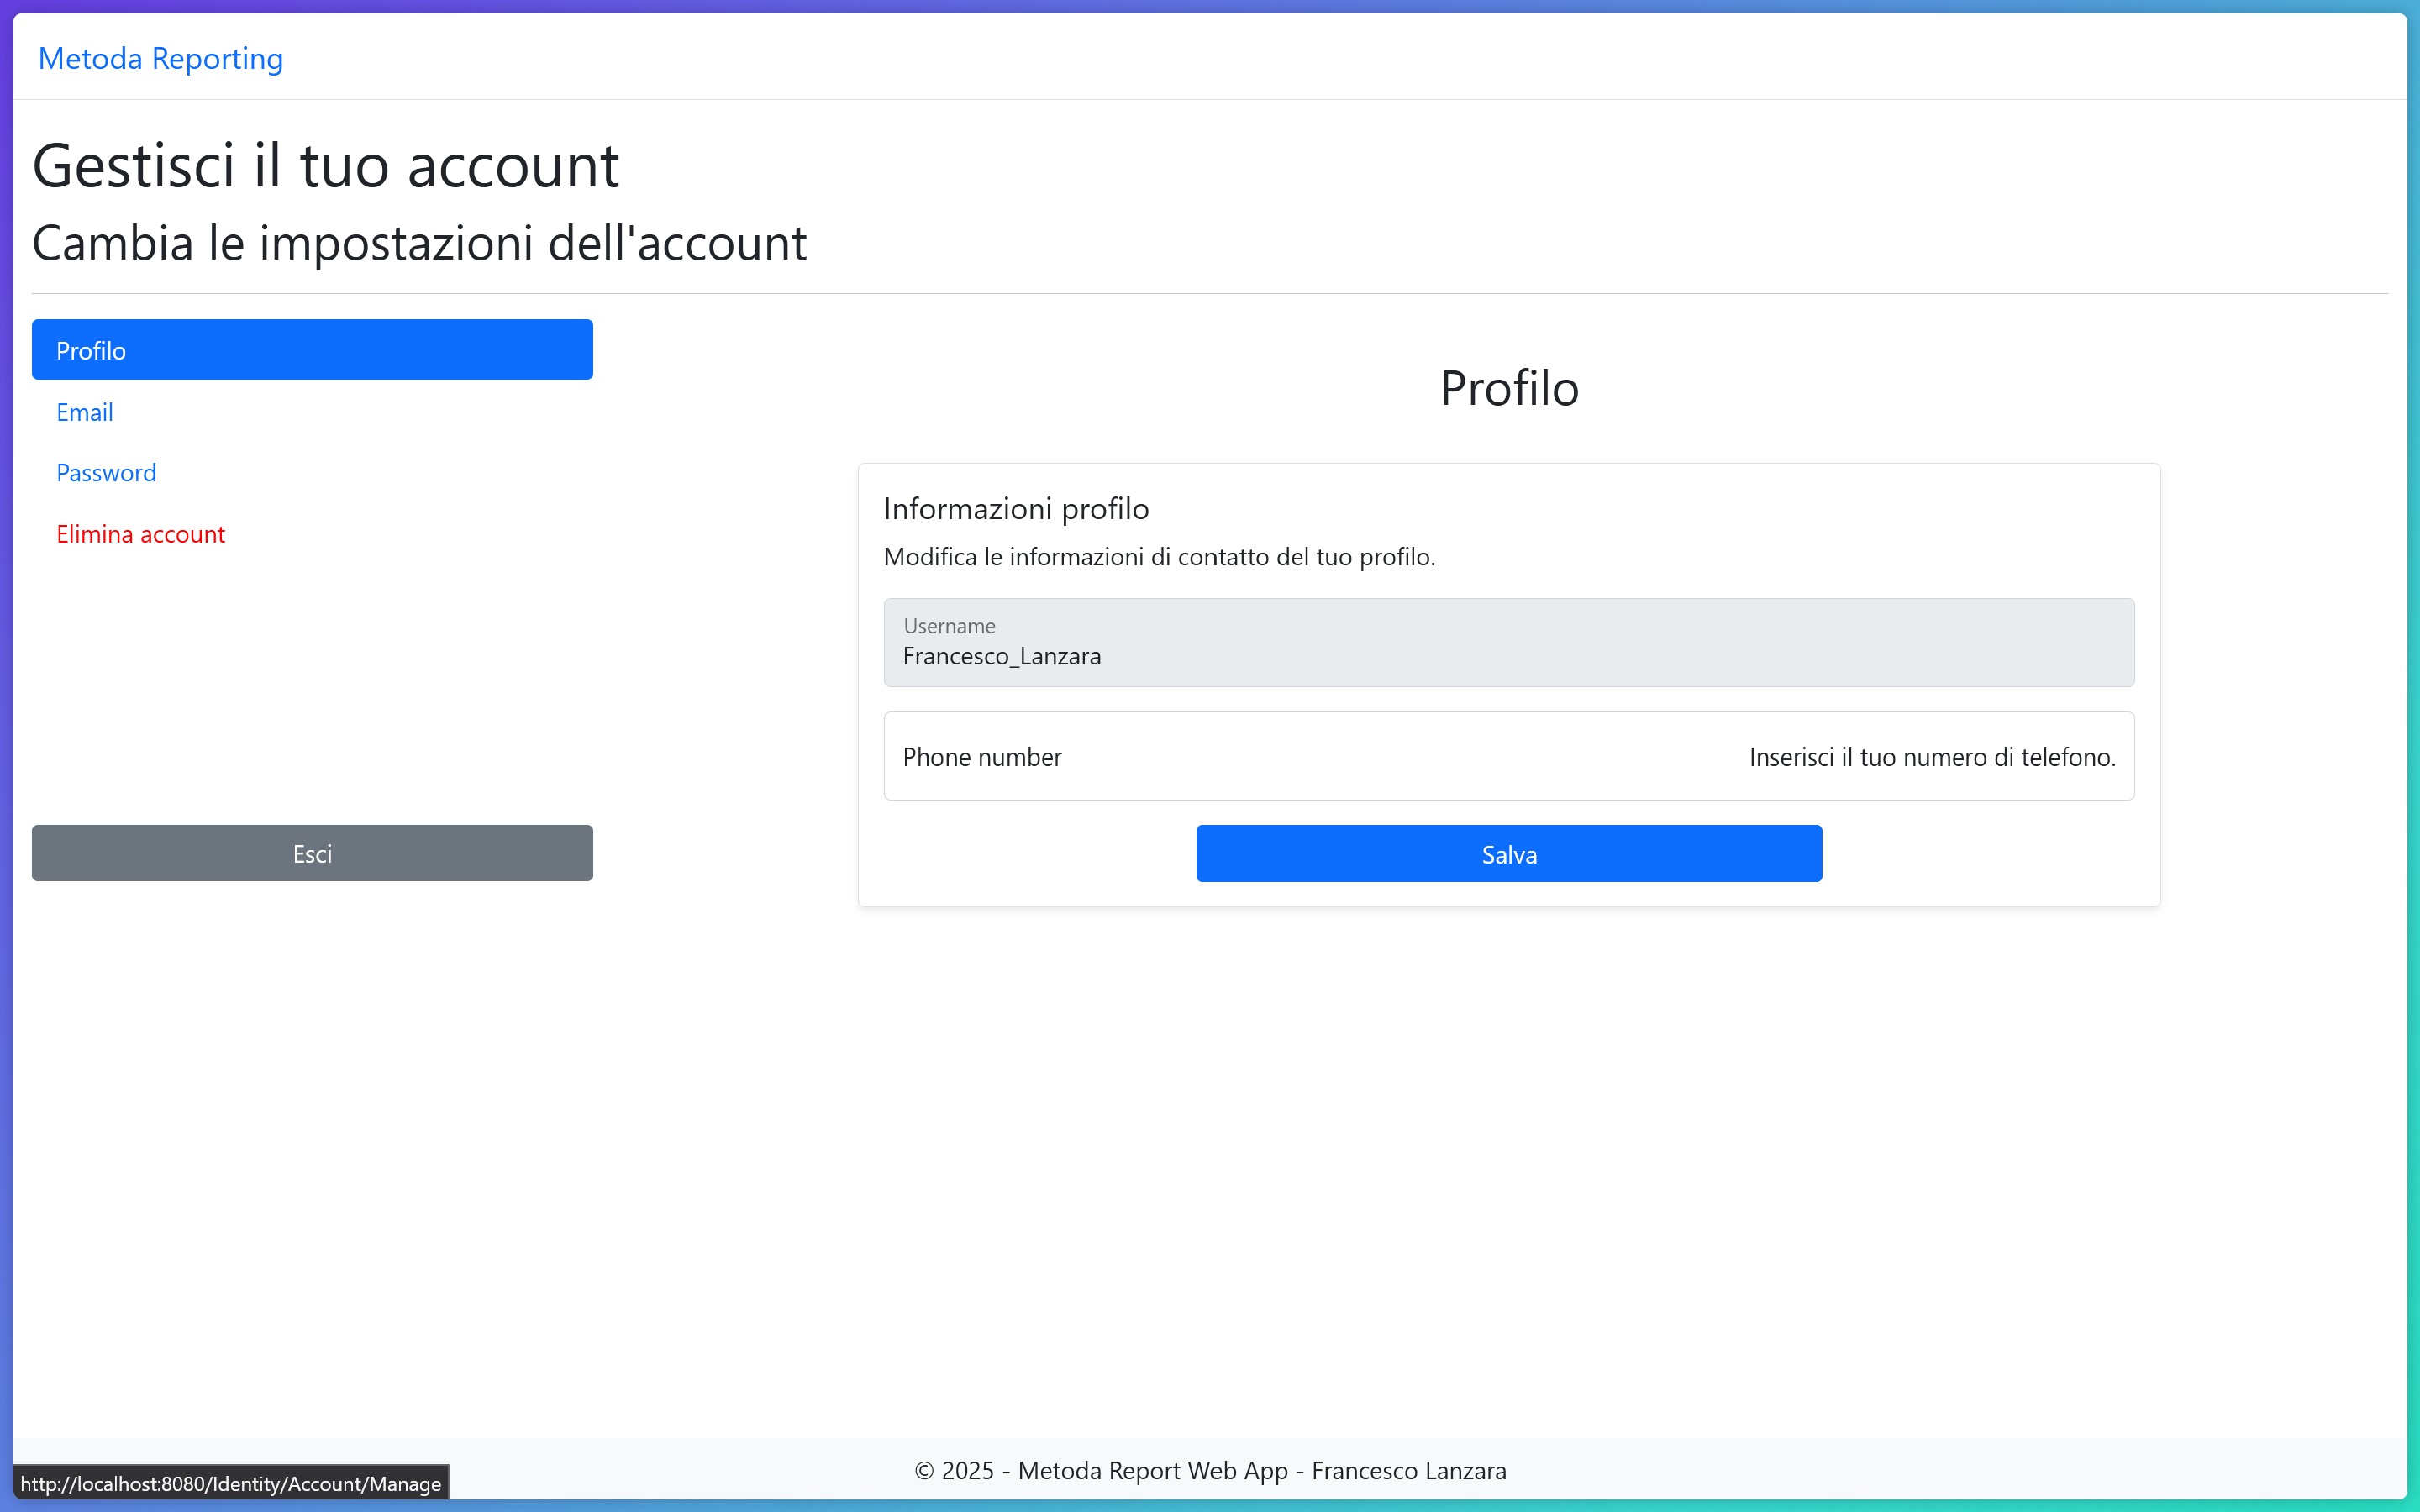
\includegraphics[width=15.5cm]{fig/screen_manage.png}
        \caption[Schermata gestione utente]{La schermata di gestione account. Contiene le sezioni \emph{profilo, email, password}. E' da questa schermata inoltre che l'utente può effettuare il \emph{logout} ed \emph{eliminare} l'account, i dati a esso assiciati e i documenti da esso generati.}
\end{figure}

In aggiunta a un sistema di refresh automatico dei token, tale sistema consente all'utente di accedere a tutti i microservizi protetti dell'architettura senza preoccuparsi di dover effettuare nuovi login, garantendo un'esperienza utente fluida e sicura che ignora la suddivisione dell'architettura in container distinti.

\subsection{Web API}
Il progetto \emph{WebAPI} implementa il microservizio che espone le API RESTful per la generazione automatica dei report e il loro salvataggio nella sezione dello storage dedicata all'utente: infatti, l'API è protetta dal gateway e pertanto risulta accessibile solo previa autenticazione.
Per realizzare tale servizio si è fatto uso del framework \emph{ASP.NET Core Web API}, che consente di creare API RESTful in modo semplice e veloce.

Come accennato in precedenza, tale microservizio ospita il motore di generazione automatica dei report, i cui moduli sono referenziati nel progetto.
Lo stato persistente è mantenuto su un \emph{named volume Docker}, su cui un database SQLite (il cui schema si fonda sul model fornito dal progetto condiviso \emph{UserDocuments}) memorizza i metadati sui documenti generati, associandoli agli utenti mediante il loro \texttt{SubjectId} (identificativo univoco fornito da OpenID Connect), mentre i file stessi sono salvati su file system, con una struttura di cartelle che li organizza per utente e data di creazione. Come prospettiva futura, si dovrebbe aggiungere un sistema di gestione dello spazio utilizzato, come una \emph{policy} di eliminazione automatica dei documenti più vecchi o un limite massimo di spazio utilizzabile per utente, per evitare che lo storage cresca indefinitamente.

Un Controller API astratto implementa, tra gli altri, i due metodi di base necessari alla generazione dei documenti, per l'esportazione rispettivamente in formati PDF ed Excel (\texttt{.xlsm}), che possono essere chiamati dai controller concreti apponendo i tipi parametrici adeguati (tra quelli disponibili del motore di reportistica) al fine di specificare categoria di report e \emph{data source} (per il testing sono state utilizzate classi statiche di tipo \texttt{-FakeData} predisposte dal modulo di test del motore di reportistica) e ottenere il report desiderato con un approccio semplice e modulare. Un ulteriore metodo è messo a disposizione per il \emph{retrieval} dei documenti precedentemente generati dall'utente e presenti in storage: come vedremo a breve, tale metodo è utilizzato dal client MVC per popolare una lista di documenti recenti con link predisposti per il download degli stessi.

La generazione dei documenti avviene in modo asincrono, con la creazione di un nuovo task per ogni richiesta, in modo da non bloccare il thread principale del server e consentire la gestione di più richieste contemporaneamente. Una volta completata la generazione, il documento viene salvato nello storage e i metadati vengono aggiornati nel database.

Essendo il principale incaricato della generazione dei report, il microservizio Web API istanzia un Hub SignalR per l'aggiornamento in tempo reale sullo stato di generazione dei report. In questo modo, quando la generazione di un documento viene richiesta dal client MVC, esso si iscrive all'hub; il controller della Web API associa all'oggetto report un \texttt{ReportProgress}, classe del motore di reportistica, che in maniera nativa consente di associare una \emph{callback} al progresso nella fase di generazione. Impostando come callback la procedura di emissione di un evento SignalR all'utente, questo può visualizzare a schermo notifiche in tempo reale sulla percentuale di avanzamento dell'operazione richiesta.

Tutti i controller concreti per la generazione espongono endpoint \texttt{GET} alla route URL \url{{dominio}/api/{CategoriaReport}/{pdf|excel}}, e si limitano a restituire in maniera asincrona il risultato del metodo generico ereditato, specificando i parametri di tipo adeguati. Ad esempio, per generare un report di tipo \emph{MonthlyReport} (Report Analitico per Controparte) in formato PDF, il client deve invocare l'endpoint
\url{{dominio}/api/MonthlyReport/pdf}, ottenendo in risposta il file generato.

Un ultimo controller che non riguarda la generazione è esposto all'endpoint \url{{dominio}/internal/userdocs}, e rappresenta l'insieme di api intese per uso amministrativo nell'ambito del motore di reportistica. Tale endopoint interno non è esposto dal gateway, e allo stato corrente del progetto consente di eliminare tutti i documenti e i dati associati a un utente: questa operazione è richiesta dal microservizio AuthServer al momento della conferma di eliminazione dell'account da parte dell'utente: si rispetta così il principio di \emph{data minimization}, non conservando dati personali dell'utente oltre il tempo necessario.
Il controller interno, in' ipotetica evoluzione futura del progetto in un ambiente distribuito, dovrebbe essere trasferito nel microservizio di reportistica separato, come discusso in precedenza, accanto al modello di dati correntemente importato dal progetto condiviso \emph{UserDocuments}.

Infine, \emph{WebAPI} utilizza il progetto condiviso \emph{UserDocuments}, che definisce il modello di dati per i documenti generati e i metadati ad essi associati, in modo da poter interagire con il database SQLite in modo tipizzato e sicuro.

\subsection{Web App}
Il progetto \emph{WebApp MVC} implementa il microservizio che ospita l'interfaccia grafica dell'applicazione, e si basa sul framework ASP.NET Core MVC. Tale interfaccia consente all'utente di interagire con l'architettura, richiedendo la generazione dei report e visualizzando i documenti generati dall'utente in precedenza, che come per la Web API sono memorizzati in uno storage del server avvalendosi della tecnologia \emph{EntityFramework Core}. Infatti, come accennato in precedenza il client MVC non comunica direttamente con il microservizio di reportistica, ma effettua un redirecting verso gli endpoint esposti dalla Web API per la generazione dei documenti; l'accesso ai documenti generati in precedenza è invece indipendente, poiché il volume che ospita i documenti e il db per i metadati associati è condiviso fra i due microservizi, così da non sovraccaricare il container Web API quando possibile. Come spiegato in precedenza, tale articolazione che sembra voltare le spalle al principio di \emph{SoC} (\emph{Separazione delle Responsabilità}) è una conseguenza di una scelta progettuale consapevole, quella di inglobare il motore di reportistica nel microservizio della Web API, che in un contesto di sviluppo professionale e distribuito sarebbe stata evitata.

L'interfaccia grafica è stata realizzata con l'ausilio del framework \emph{Bootstrap}, al fine di creare layout responsive e gradevoli alla vista in modo semplice e veloce, grazie a una vasta libreria di componenti predefiniti e personalizzabili. L'uso di tale framework facilita inoltre il mantenere un aspetto coerente e professionale in tutte le pagine dell'applicazione, migliorando l'esperienza utente.

L'architettura MVC consente di separare chiaramente le responsabilità tra modello, vista e controller, facilitando la manutenzione e l'estensibilità del codice. I controller gestiscono le richieste HTTP, interagiscono con i modelli per recuperare o modificare i dati e selezionano le viste appropriate per la presentazione all'utente.

Le view principali esposte dal prototipo, oltre a quelle di default fornite dal template e personalizzate per l'applicazione, sono la home page e la pagina del profilo utente.
La home page è esposta all'endpoint radice del dominio, e consente all'utente di richiedere la generazione di nuovi report mediante una lista di \emph{card}, una per ogni categoria di report generabile, ognuna dotata due pulsanti, uno per ciascun formato supportato (PDF ed Excel).
Una checkbox (la cui preferenza è memorizzata associandola al profilo utente) consente di determinare se aprire direttamente i report richiesti in una nuova scheda del browser, o se generarli e renderli successivamente disponibili dall'elenco dei documenti dell'utente. Grazie alla connessione del client MVC con l'hub SignalR esposto dalla Web API, la home viene aggiornata in tempo reale sullo stato di avanzamento della generazione del documento richiesto mediante una progress bar: al termine della generazione un \emph{toast} (notifica popup) in alto a sinistra dello schermo informa l'utente del completamento dell'operazione, consentendogli opzionalmente di aprire il file generato.

\begin{figure}[H]
        \centering
        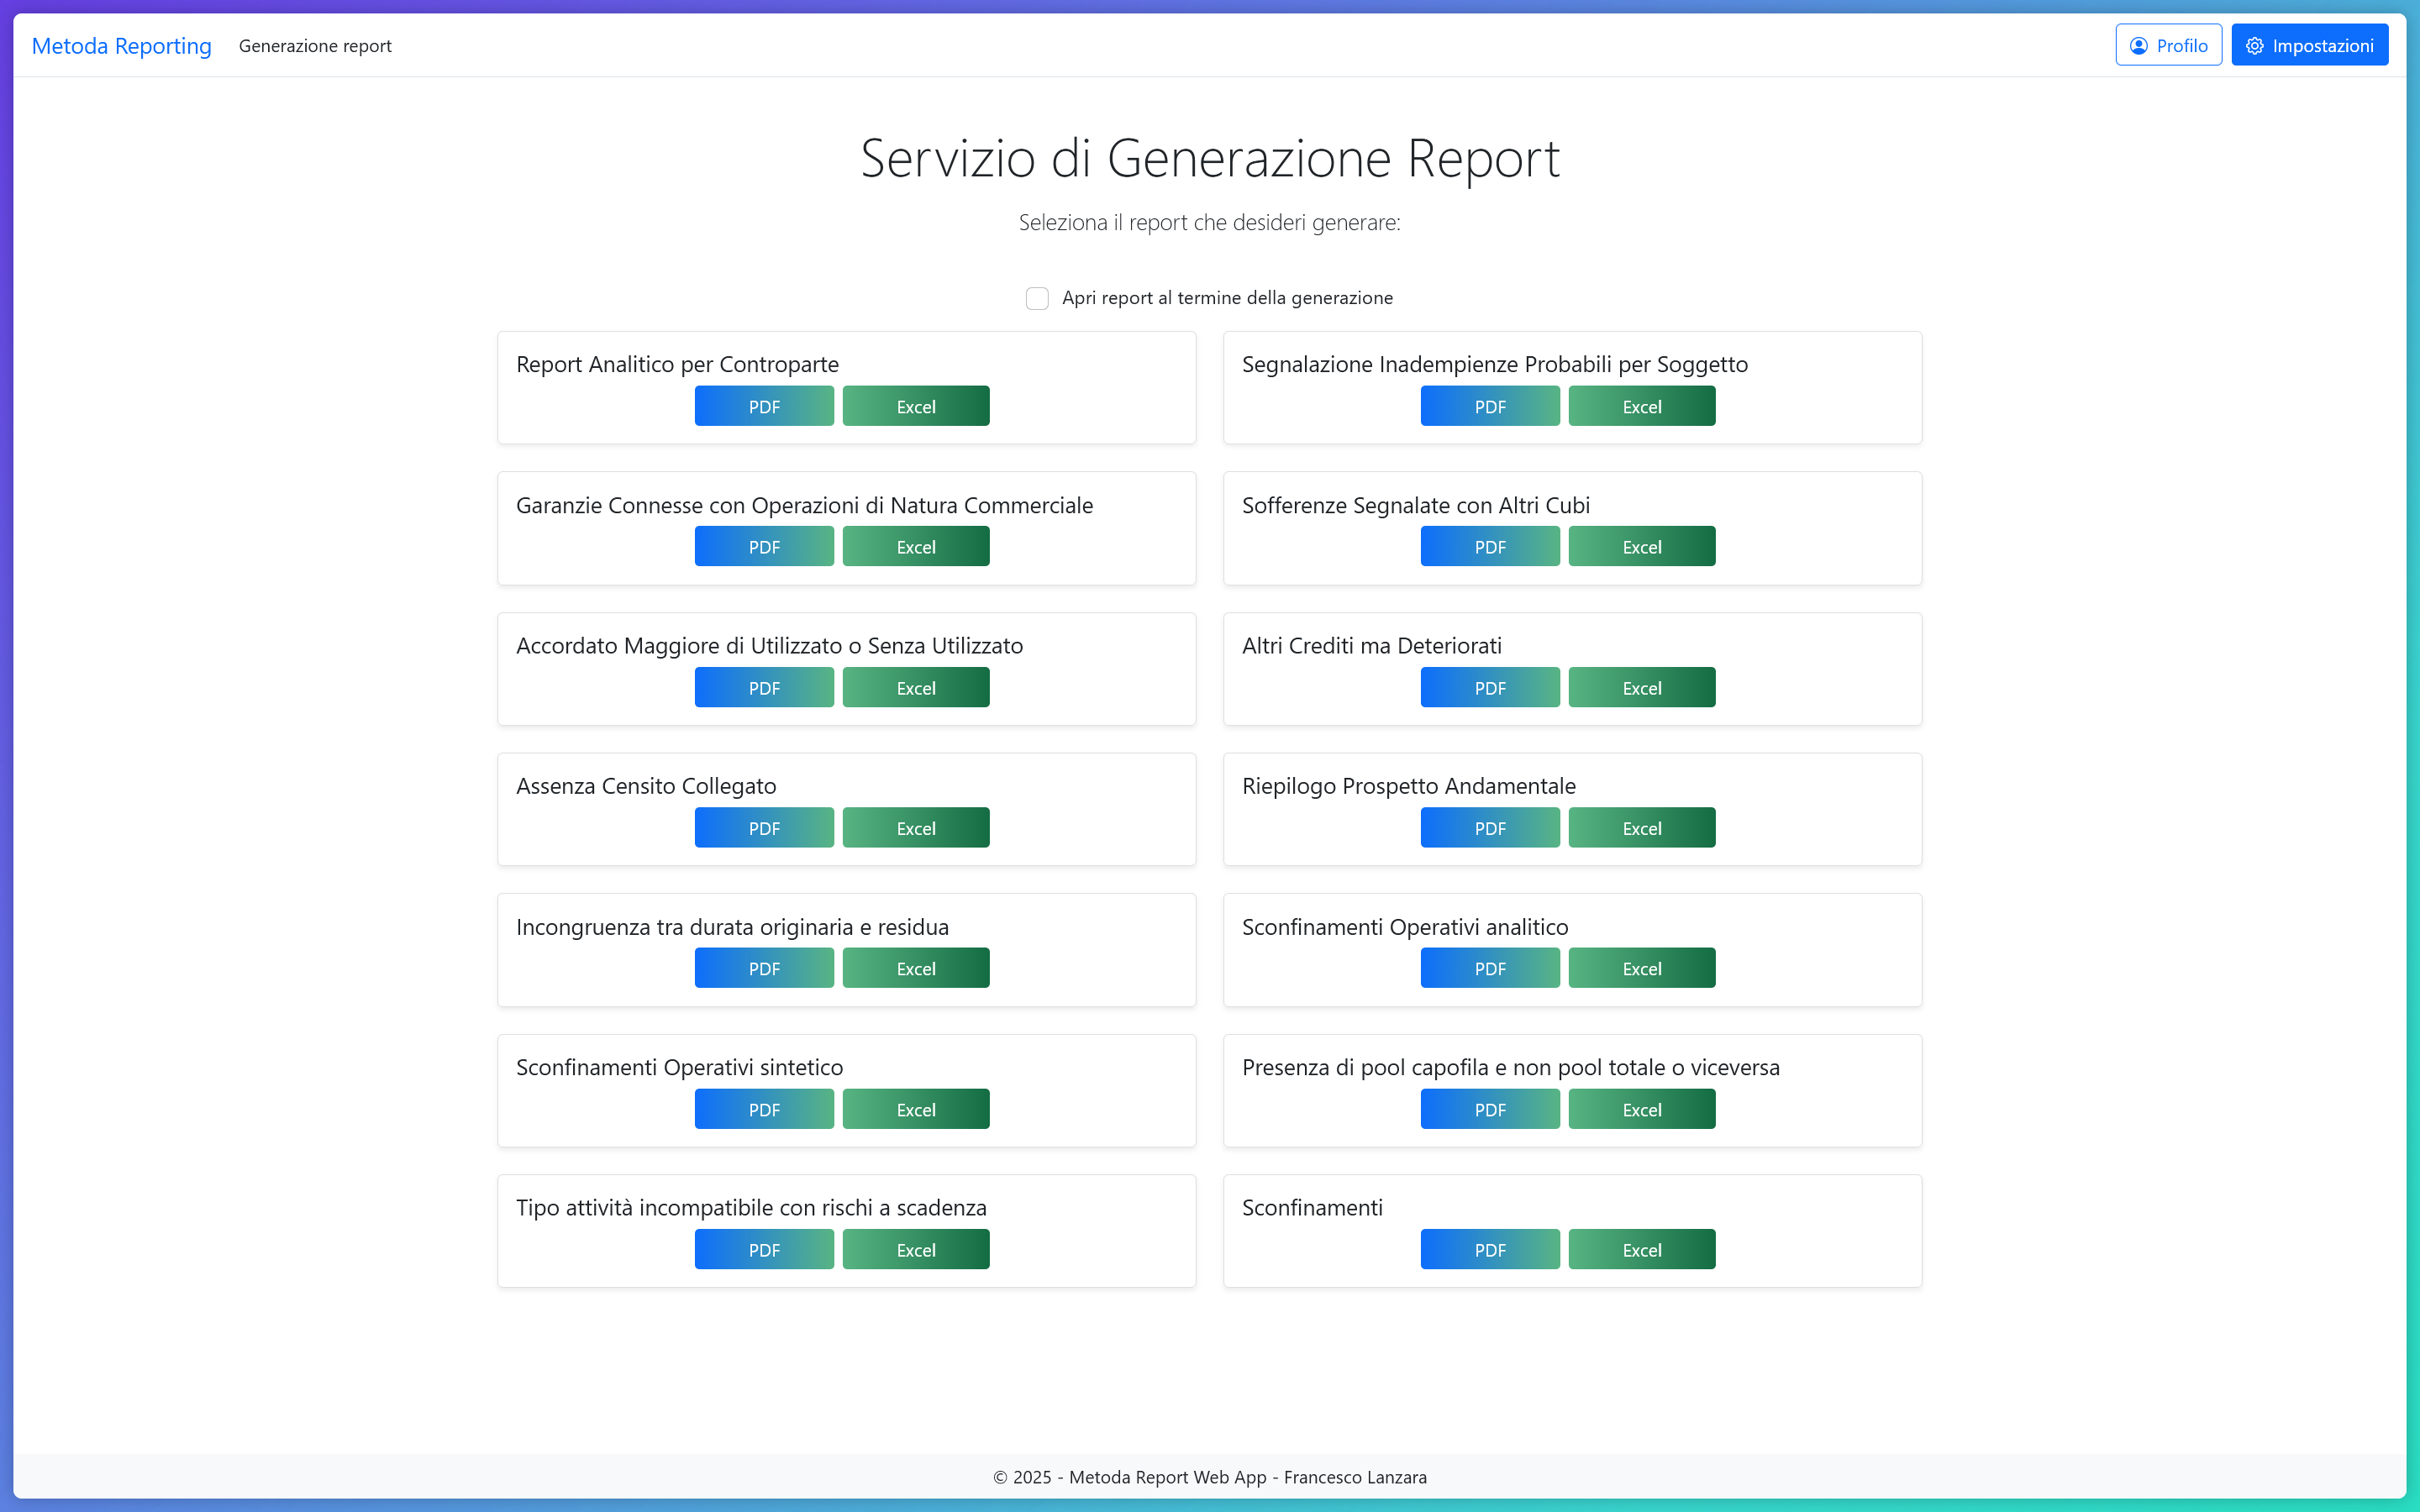
\includegraphics[width=15.5cm]{fig/screen_home.png}
        \caption[Schermata home]{La schermata principale dell'applicazione. Da questa schermata è possibile richiedere la generazione di nuovi report.}
\end{figure}

La pagina del profilo utente, accessibile dal menu in alto a destra, consente di visualizzare i dati relativi al profilo e l'elenco dei documenti generati in precedenza, con link per il download diretto e informazioni sui metadati associati (data di creazione, formato, categoria). Per la popolazione della lista dei documenti, il client MVC agisce indipendentemente dalla Web API, usufruendo del model \emph{EntityFramework Core} ottenuto referenziando il progetto condiviso \emph{UserDocuments}. In questo modo, il client può accedere direttamente al database SQLite condiviso per recuperare i documenti associati all'utente autenticato, senza dover passare per la Web API, alleggerendo il carico su quest'ultima e migliorando le prestazioni complessive dell'applicazione.
Un pulsante di logout consente di disconnettere l'utente, che viene reindirizzato alla pagina di login dell'AuthServer, mentre è possibile raggiungere la sezione di gestione dell'account (e indirettamente tutte le altre pagine che riguardano l'identità dell'utente, come login e registrazione) grazie al pulsante \emph{Impostazioni} posto accanto a quello del profilo sulla barra di navigazione superiore.

\begin{figure}[H]
        \centering
        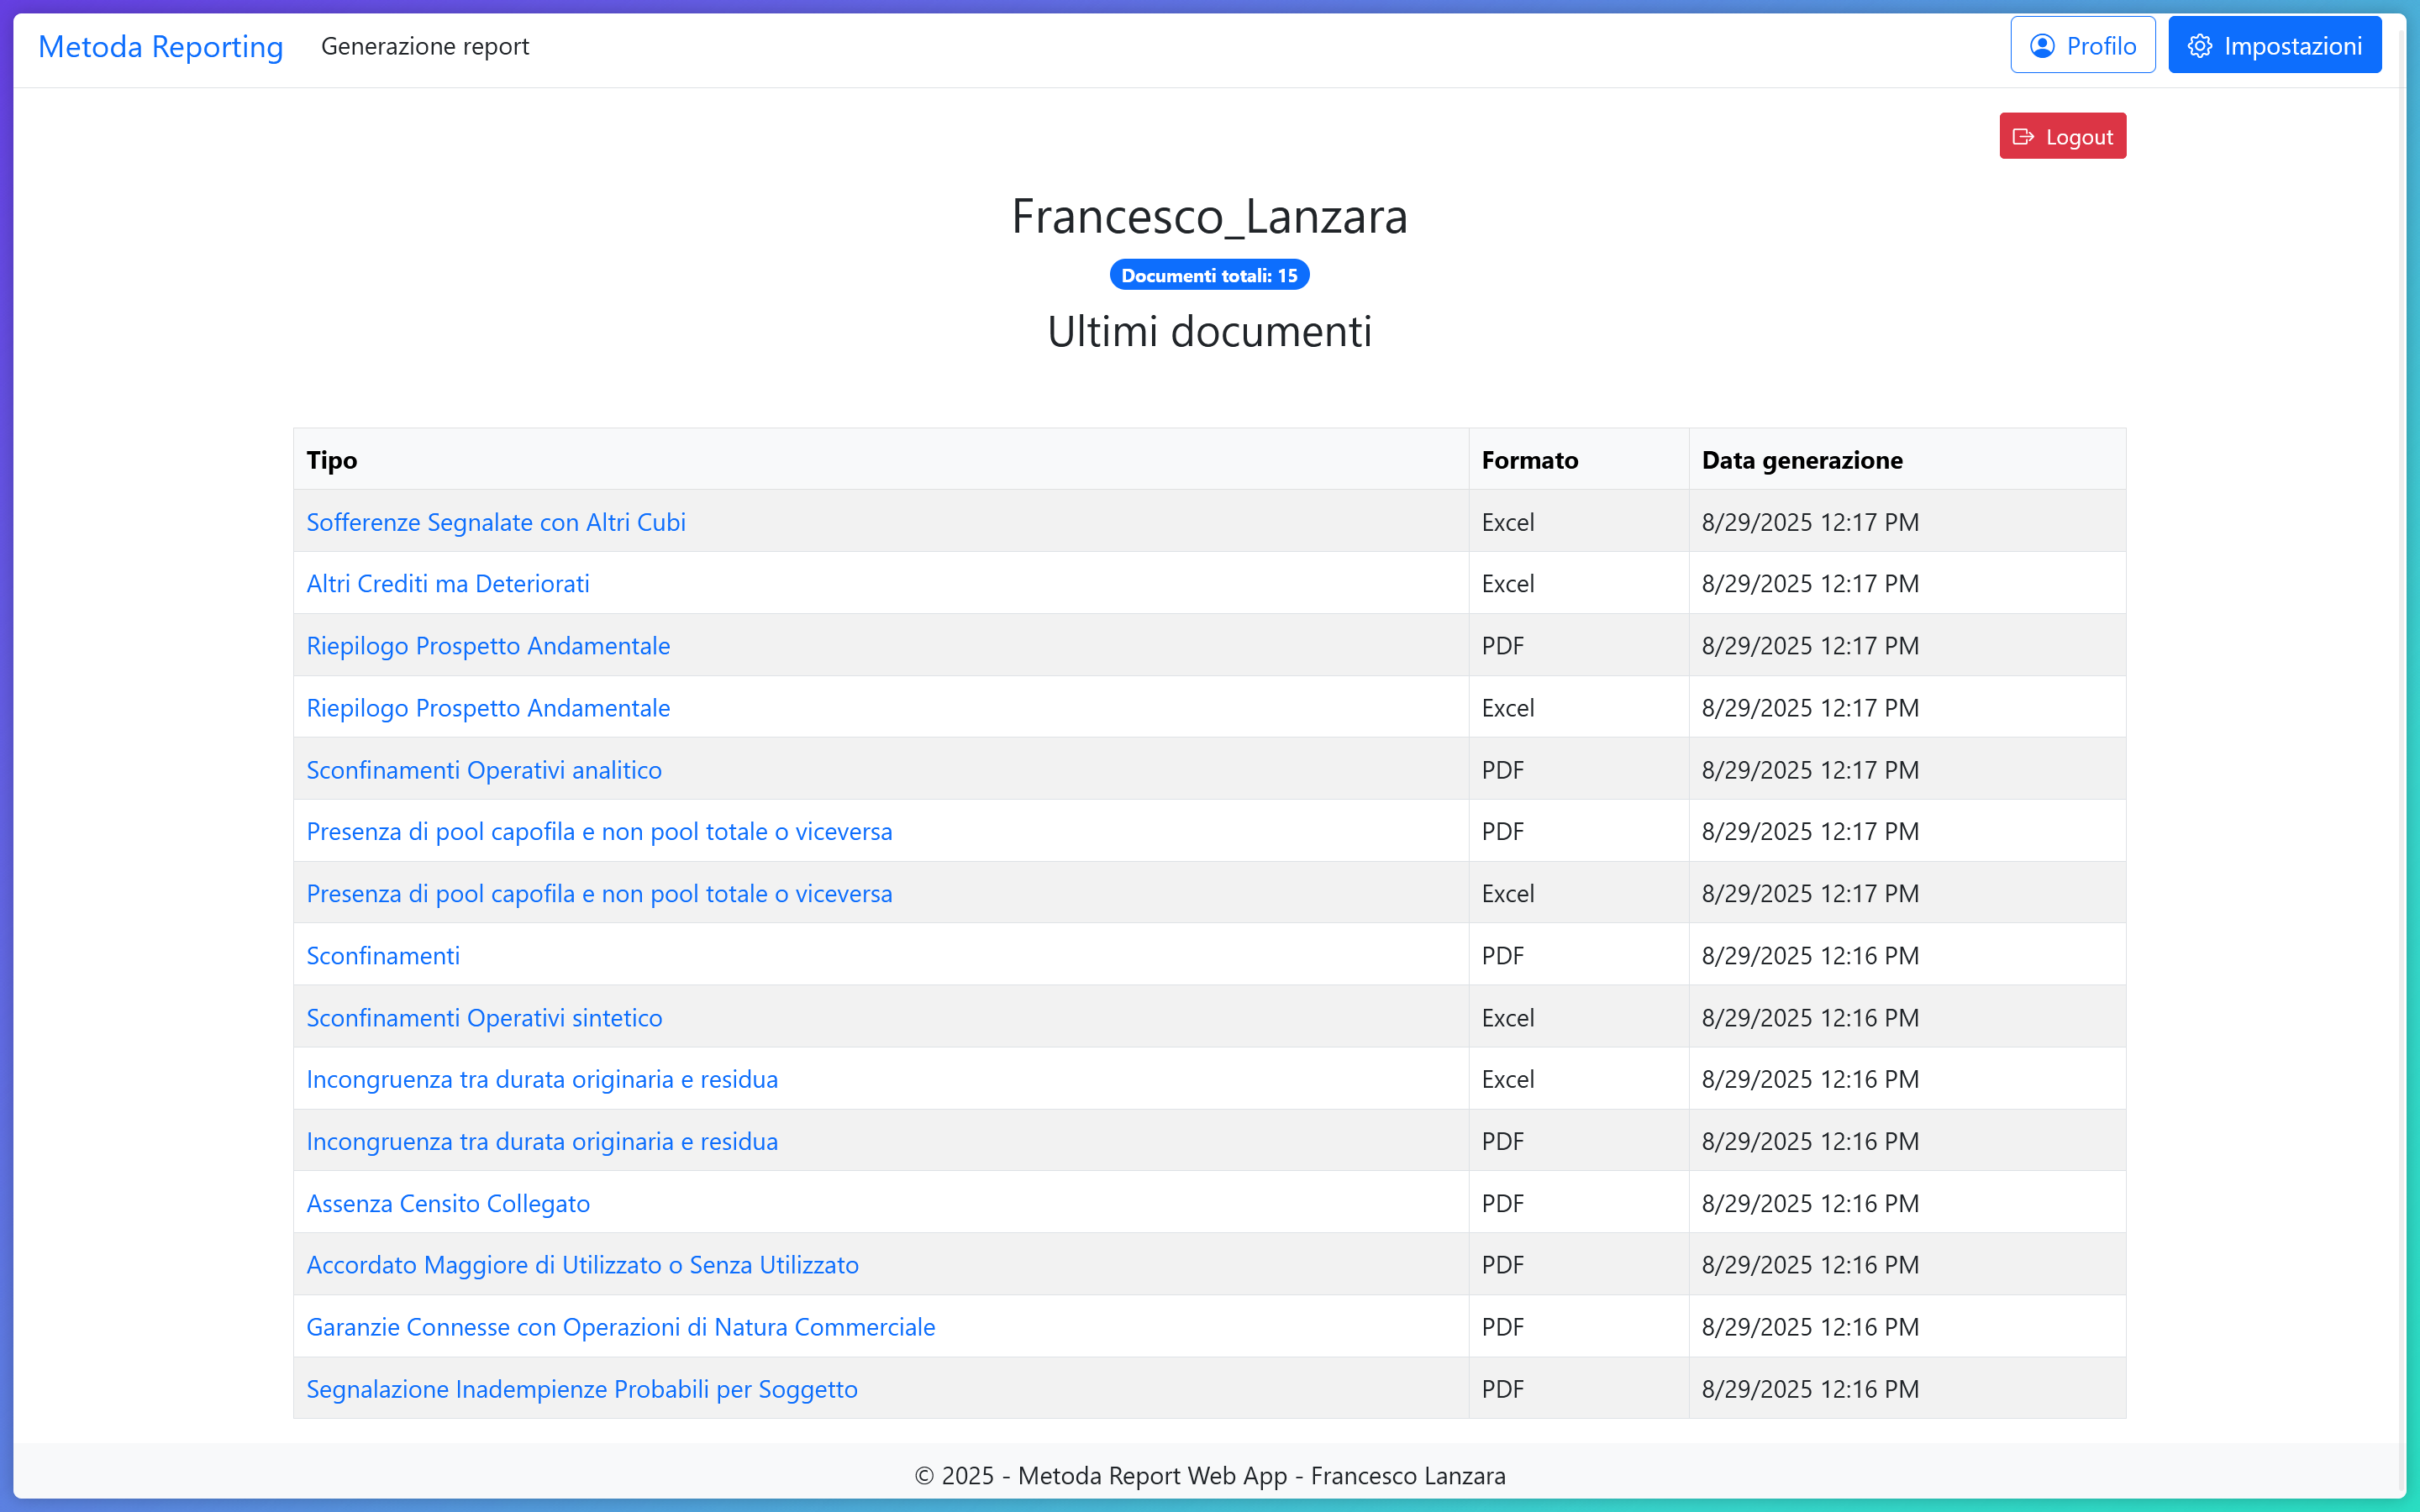
\includegraphics[width=15.5cm]{fig/screen_profile.png}
        \caption[Schermata profilo]{La schermata del profilo utente. Da questa schermata è possibile scaricare i documenti generati in precedenza, effettuare il logout e accedere alla gestione dell'account.}
\end{figure}

Nonostante l'autenticazione dell'utente sia delegata al tier superiore del gateway API, il client MVC è configurato per generare e validare \emph{cookie Anti-Forgery} per proteggere le richieste \texttt{POST} (eseguite alla selezione di uno dei pulsanti di generazione report) da attacchi di tipo \emph{Cross-Site Request Forgery} (CSRF), pratica che rientra nelle best practice per la sicurezza delle applicazioni web.

\subsection{UserDocuments}
Come accennato in precedenza, \emph{UserDocuments} è un progetto condiviso .NET che usufruisce del pacchetto \emph{EntityFramework Core} per definire in maniera semplice e potente il modello di dati per i report generati dagli utenti e per i metadati ad essi associati. Tale progetto è referenziato sia dal microservizio Web API, che lo utilizza per interagire con il database SQLite durante la generazione dei report (anche per conto della web app), sia dal client MVC, che lo impiega per accedere direttamente al database e recuperare i report associati all'utente autenticato.

Esso consta di due \emph{namespace} principali: \emph{Models} e \texttt{Services} (i \emph{namespace} sono uno degli elementi che consentono di organizzare gerarchicamente il codice in .NET).
In \texttt{Models} troviamo ciò che riguarda la definizione del modello dei dati:
\begin{itemize}
        \item \texttt{UserDoc} rappresenta il modello dei dati dei report generati, esponendo proprietà tra cui il \emph{GUID} (identificativo univoco globale) dell'utente che ha generato il documento (coordinato con il database dell'Identity Provider \emph{AuthServer}), metadati sul documento e il percorso nel file system in cui è salvato.
        \item \texttt{UserDocsDbContext} estende la classe \texttt{DbContext} di \emph{EntityFramework Core}: questo è il modo in cui quest'ultimo strumento riesce a mappare le classi C\# come parte dello schema del database relazionale, consentendo come già detto di interagire con esso in modo tipizzato e sicuro.
        In questo caso specifico, l'esposizione di una proprietà \texttt{DbSet<UserDoc>} consente a \emph{EF} di creare e gestire la tabella dei documenti generati dagli utenti, fornendo metodi per l'inserimento, l'aggiornamento, la cancellazione e la query dei record generati automaticamente a partire dalla classe di modello fornita.
        \item \texttt{DocumentContent} racchiude una \emph{sealed hierarchy} di possibili valori, uno per ogni categoria di report supportata, che esposti come elenco di proprietà statiche consente di specificare in modo tipizzato e centralizzato la categoria di report da generare quando si invoca l'API della Web API. Si evitano inoltre stringhe \emph{hardcoded} sparse per il codice specificando qui tutti i metadati necessari alla manipolazione dei titoli e dei \emph{filename}: ciò aumenta la modularità e manutenibilità del codice, fornendo un unico file sorgente in cui apportare tutti gli aggiornamenti che riguardano il dominio applicativo (come le categorie dei report e la loro denominazione).
        Questa soluzione, oltre a ridurre la possibilità di bug dovuti a errori di battitura (viene in aiuto allo sviluppatore il sistema di \emph{IntelliSense} dell'IDE, che fornisce suggerimenti e completamenti automatici basati sulla gerarchia fornita), permette di sfruttare al meglio l'interazione di \emph{Razor} con l'ecosistema \emph{C\#/.NET}.
        Come spiegato in precedenza, il framework \emph{ASP.NET Core MVC} consente di creare viste dinamiche che interagiscono con la \emph{codebase} in modo fluido e naturale, grazie alla sintassi \emph{Razor}, che permette di mescolare HTML e C\# in un unico file.
        Grazie a tale caratteristica, ad esempio, l'elenco di \emph{card} nella home page del client MVC viene popolato dinamicamente iterando sull'elenco di categorie esposto da \texttt{DocumentContent}, evitando di dover ripetere manualmente il codice HTML per ogni categoria di report supportata.
\vspace{0.5cm}

        \begin{lstlisting}[language={[Sharp]C}, caption={[Estratto della view dell'homepage] Estratto della \emph{view} principale dell'interfaccia web, a dimostrazione della potenza di Razor nell'integrazione di logica e markup per il rendering dinamico.}, label=lst:indexcshtml]
@foreach (var report in reports)
{
    [...]
    <div class="card-body d-flex flex-column">
           <h5 class="card-title">@report.Title</h5>
           <div class="mt-auto d-flex justify-content-center gap-0">
           @foreach (var format in formats)
           {
                   <form class="report-form" asp-controller="Home" asp-action="Index" method="post">
                   @Html.AntiForgeryToken()
                   <input type="hidden" name="docCategory" value="@report.ApiName" />
                   <input type="hidden" name="format" value="@format.Ext" />
                   <input type="hidden" name="openReport" value="false" />
                   <button type="submit" class="btn me-2 @format.Css px-5">@format.Label</button>
                   </form>
           }
           </div>
    </div>
    [...]
}
\end{lstlisting}
\end{itemize}

Invece, in \emph{Services} troviamo la classe \texttt{DocumentStorageService}, utilizzata dai controller di Web API e Web App per interagire in maniera standardizzata mediante metodi di accesso asincroni e altri tool di utility. I metodi sono pensati per integrare completamente la logica di gestione delle richieste, per cui presentano una \emph{signature} (\emph{firma}, ossia la definizione del metodo) adatta a gestire le principali operazioni che ci si attende dai controller: per questo motivo, non è necessario eseguire il \emph{wrapping} di tali metodi in altra logica, ma è possibile utilizzarli direttamente, specificando i parametri del caso per ottenere il risultato desiderato.
Un esempio sono i metodi \texttt{GenerateAndSavePdfReportAsync} e \texttt{GenerateAndSaveExcelReportAsync}, che incapsulano l'intera logica di generazione e salvataggio dei report, restituendo una \texttt{Task} che rappresenta il documento generato e i suoi metadati. In questo modo, i controller possono ottenere l'effetto collaterale del salvataggio in memoria, prima di restituire gli oggetti che nella gerarchia ASP.NET Core gestiscono in maniera asincrona la risposta HTTP al client contenente il file generato.

\subsection{Global}
Il progetto \emph{Global} è un progetto di utilità che fornisce funzionalità condivise e helper per conferire modularità e manutenibilità agli altri progetti della soluzione. In particolare, esso contiene:
\begin{itemize}
        \item la classe statica Domain, che contiene proprietà e metodi per l'elaborazione di valori come \emph{host}, \emph{schema} e \emph{porta} e l'interpolazione dinamica dei path URL d'interesse per l'applicativo;
        \item una classe d'eccezione \texttt{InvalidConfigurationException}, che scandisce gli eventi di errata configurazione dell'applicativo, come la mancanza di variabili d'ambiente o oggetti di \texttt{appsettings.json} necessari essenziali per il corretto funzionamento dei microservizi;
        \item la classe \texttt{ConfigurationExtractor}, istanziata da tutti i progetti \emph{ASP.NET} nel file d'avvio \texttt{Program.cs} per usufruire dei metodi da essa forniti per il \emph{retrieval} \emph{type-safe} e \emph{null-checked} (pena il lancio dell'eccezione descritta sopra) delle configurazioni del microservizio, garantendo che sviste nella modifica di file quali \texttt{Dockerfile}, \texttt{docker-compose.yml} o \texttt{appsettings.json} vengano prontamente individuate e segnalate, evitando scomode \texttt{NullReferenceException} a \emph{runtime} che risultano in \emph{stacktrace} verbose e per nulla esaustive in fase di debug.
\end{itemize}

\subsection{Docker Compose}
Il progetto \emph{Docker Compose} è responsabile della definizione e gestione dei container Docker per l'applicativo.
Il file fondamentale è \texttt{docker-compose.yml}, che come accennato nei capitoli precedenti definisce i servizi, le reti e i volumi necessari per l'esecuzione dell'applicativo in ambiente containerizzato. In esso sono specificati i dettagli di ogni microservizio, come il \texttt{Dockerfile} da utilizzare per la build, le porte esposte e condivise in rete privata, le variabili d'ambiente e le dipendenze tra i servizi.
I servizi definiti sono 4, uno per ogni microservizio descritto in precedenza: \emph{gateway}, \emph{authserver}, \emph{rest} e \emph{mvcclient}.
Ognuno di essi è configurato per utilizzare un'immagine Docker basata su \emph{Windows nanoserver-1809} con runtime .NET 8 ASP.NET; \emph{gateway} è l'unico container a fare \emph{port forwarding} sulla porta 8080 della macchina host, esponendo l'applicativo all'esterno, mentre gli altri container comunicano fra loro in una rete privata di tipo \texttt{bridge}, isolata dalla rete host, sempre utilizzando la porta 8080.
Vengono definiti 4 \emph{named volumes}: \texttt{dpkeys} per la persistenza delle chiavi di Data Protection, \texttt{docstorage} per il salvataggio dei report degli utenti, \texttt{docmetadatadb} per il database contenente i metadati sui report e \texttt{datakeys} per salvare le chiavi di crittografia per l'Identity Server.
Nel complesso, il progetto \emph{Docker Compose} costituisce un punto singolo d'avvio per l'applicativo, consentendo una gestione centralizzata e semplificata dei container che costituiscono l'architettura a microservizi.